\documentclass[border=10pt]{standalone}

\usepackage{tikz}
\usepackage{tikzsymbols}
\usetikzlibrary{calc,patterns,shapes.geometric}

\def\centerarc[#1](#2)(#3:#4:#5){\draw[#1] ($(#2)+({#5*cos(#3)},{#5*sin(#3)})$) arc (#3:#4:#5);}

\begin{document}
	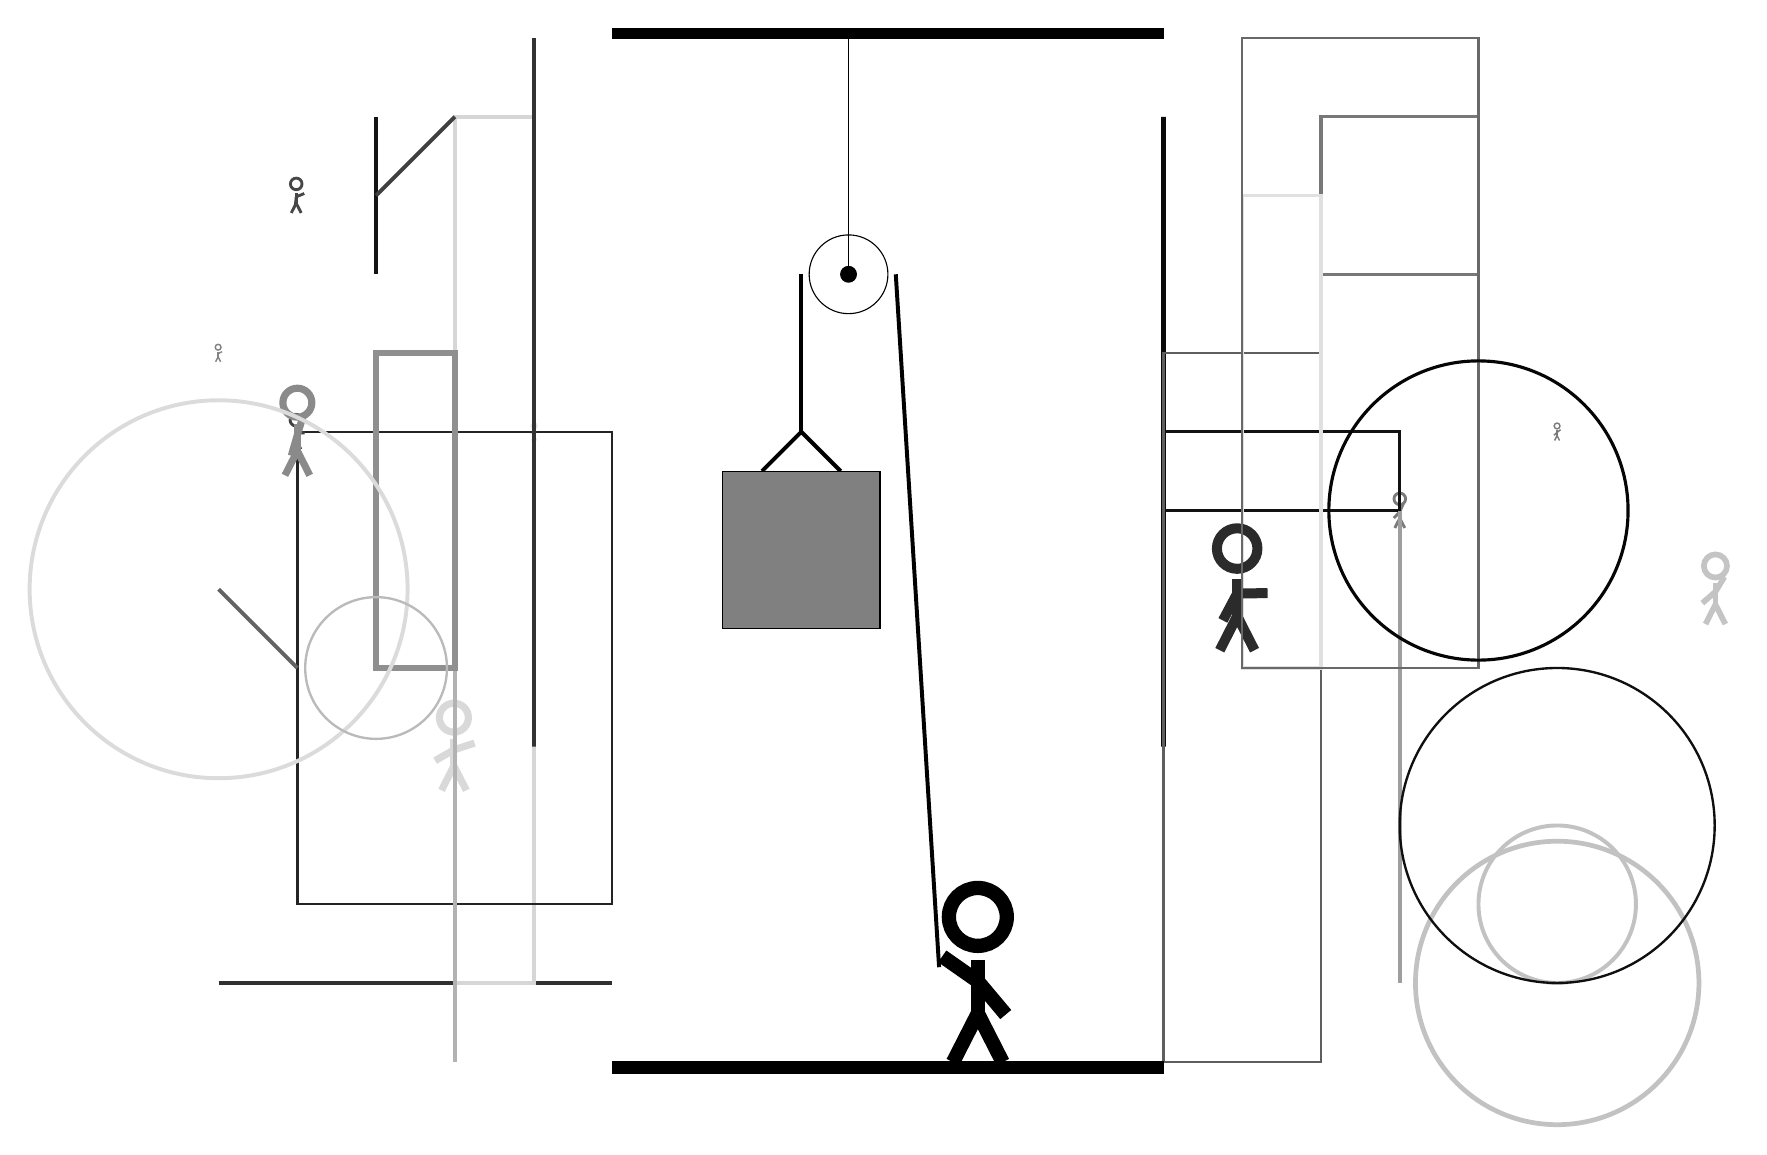
\begin{tikzpicture}
		%%%%% START %%%%%
		
		\draw[fill=black] (-2, 10) rectangle (5, 10.125);
		
		\draw[line width=0.5mm, color=black!81](-7, -2) -- (-2, -2);
		
		\node[line width=0.3mm, color=black!10] at (-3, 5) {\Strichmaxerl[1][19][78]};
		\draw[line width=0.5mm, color=black!16] (-4, -2) rectangle (-3, 9);
		\draw[line width=0.2mm, color=black!96] (6, 2) rectangle (6, 2);
		
		\draw[line width=0.6mm, color=black!96] (5, 1) rectangle (5, 9);
		\draw [line width=0.5mm, color=black!24](10, -1) circle (1.0);
		\node[line width=0.5mm, color=black!52] at (8, 4) {\Strichmaxerl[2][47][66]};
		\node[line width=0.7mm, color=black!23] at (12, 3) {\Strichmaxerl[4][41][59]};
		\draw[line width=0.5mm, color=black!58] (5, -3) rectangle (5, 4);
		\node[line width=0.2mm, color=black!52] at (10, 5) {\Strichmaxerl[1][42][37]};
		\draw[line width=0.5mm, color=black!92](-5, 9) -- (-5, 7);
		\draw[line width=0.3mm, color=black!86] (-2, -1) rectangle (-6, 5);
		\draw[line width=0.4mm, color=black!93] (5, 4) rectangle (8, 5);
		
		\draw[line width=0.4mm, color=black!53] (7, 7) rectangle (9, 9);
		\node[line width=0.4mm, color=black!15] at (-4, 1) {\Strichmaxerl[5][30][18]};
		\draw[line width=0.3mm, color=black!63] (5, 6) rectangle (7, -3);
		
		\node[line width=0.3mm, color=black!75] at (-6, 5) {\Strichmaxerl[2][86][1]};
		\node[line width=0.2mm, color=black!49] at (-7, 6) {\Strichmaxerl[1][86][27]};
		\node[line width=0.3mm, color=black!46] at (-6, 5) {\Strichmaxerl[5][74][73]};
		\draw[line width=0.5mm, color=black!38](8, 4) -- (8, -2);
		\draw[line width=0.5mm, color=black!30](-4, 3) -- (-4, -3);
		
		\draw[line width=0.4mm, color=black!12] (7, 8) rectangle (6, 2);
		\draw [line width=0.6mm, color=black!24](10, -2) circle (1.8);
		\draw[line width=0.5mm, color=black!80] (-3, 1) rectangle (-3, 10);
		\draw[line width=0.5mm, color=black!75](-4, 9) -- (-5, 8);
		
		\draw[line width=0.7mm, color=black!44] (-4, 2) rectangle (-5, 6);
		\draw[line width=0.5mm, color=black!61](-6, 2) -- (-7, 3);
		\node[line width=0.5mm, color=black!83] at (6, 3) {\Strichmaxerl[7][62][1]};
		
		\draw[line width=0.3mm, color=black!59] (6, 2) rectangle (9, 10);
		\draw [line width=0.4mm, color=black!98](9, 4) circle (1.9);
		\draw [line width=0.5mm, color=black!14](-7, 3) circle (2.4);
		
		\draw [line width=0.3mm, color=black!27](-5, 2) circle (0.9);
		\node[line width=0.4mm, color=black!72] at (-6, 8) {\Strichmaxerl[2][84][22]};
		\draw [line width=0.3mm, color=black!94](10, 0) circle (2.0);
		
		\draw (1, 7) circle (0.5);
		\draw[fill=black] (1, 7) circle (0.1);
		\draw (1, 10) -- (1, 7);
		
		\draw[line width=0.5mm] (-0.1, 4.5) -- (0.4, 5.0) -- (0.9, 4.5);
		\draw[fill=black!50] (-0.6, 4.5) rectangle (1.4, 2.5);
		
		\draw[line width=0.5mm] (0.4, 7) -- (0.4, 5.0);
		\centerarc[line width=0.5mm](1, 7)(0:180:0.6);
		\draw[line width=0.5mm](1.6, 7) -- (2.15, -1.8);
		
		\node at (2.6, -1.9) {\Strichmaxerl[10][-35][-50]};
		
		\draw[fill=black] (-2, -3) rectangle (5, -3.15);
		
		%%%%% END %%%%%
	\end{tikzpicture}
\end{document}